%%%%%%%%%%%%%%%%%%%%%%%%%%%%%%%%%%%%%%%%%
% Beamer Presentation
% LaTeX Template
% Version 1.0 (10/11/12)
%
% This template has been downloaded from:
% http://www.LaTeXTemplates.com
%
% License:
% CC BY-NC-SA 3.0 (http://creativecommons.org/licenses/by-nc-sa/3.0/)
%
%%%%%%%%%%%%%%%%%%%%%%%%%%%%%%%%%%%%%%%%%

%----------------------------------------------------------------------------------------
%	PACKAGES AND THEMES
%----------------------------------------------------------------------------------------

\documentclass[xcolor=dvipsnames]{beamer}
\usepackage{tikz}
\usepackage{graphicx}
\usepackage{setspace}
\usepackage{fancyvrb}
\usepackage{lipsum}
\usepackage{verbatimbox}
\setbeamertemplate{background canvas}{
\begin{tikzpicture}
\node[opacity=.15]{
\hspace{3cm}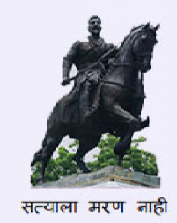
\includegraphics[height=0.8\paperheight]{logo.png}
};
\end{tikzpicture}}

\mode<presentation> {

% The Beamer class comes with a number of default slide themes
% which change the colors and layouts of slides. Below this is a list
% of all the themes, uncomment each in turn to see what they look like.
\usefonttheme[stillsansseriftext]{structurebold}

%\usetheme{default}
\usetheme{AnnArbor}
%\usetheme{Antibes}
%\usetheme{Bergen}
%\usetheme{Berkeley}
%\usetheme{Berlin}
%\usetheme{Boadilla}
%\usetheme{CambridgeUS}
%\usetheme{Copenhagen}
%\usetheme{Darmstadt}
%\usetheme{Dresden}
%\usetheme{Frankfurt}
%\usetheme{Goettingen}
%\usetheme{Hannover}
%\usetheme{Ilmenau}
%\usetheme{JuanLesPins}
%\usetheme{Luebeck}
%\usetheme{Madrid}
%\usetheme{Malmoe}
%\usetheme{Marburg}
%\usetheme{Montpellier}
%\usetheme{PaloAlto}
%\usetheme{Pittsburgh}
%\usetheme{Rochester}
%\usetheme{Singapore}
%\usetheme{Szeged}
%\usetheme{Warsaw}

% As well as themes, the Beamer class has a number of color themes
% for any slide theme. Uncomment each of these in turn to see how it
% changes the colors of your current slide theme.

%\usecolortheme{albatross}
%\usecolortheme{beaver}
%\usecolortheme{beetle}
%\usecolortheme{crane}
%\usecolortheme{dolphin}
%\usecolortheme{dove}
%\usecolortheme{fly}
%\usecolortheme{lily}
\usecolortheme{orchid}
%\usecolortheme{rose}
%\usecolortheme{seagull}
%\usecolortheme{seahorse}
%\usecolortheme{whale}
%\usecolortheme{wolverine}

%\setbeamertemplate{footline} % To remove the footer line in all slides uncomment this line
%\setbeamertemplate{footline}[page number] % To replace the footer line in all slides with a simple slide count uncomment this line

%\setbeamertemplate{navigation symbols}{} % To remove the navigation symbols from the bottom of all slides uncomment this line
\setbeamercolor{frametitle}{fg=white,bg=blue}
\setbeamercolor*{title}{bg=blue,fg=white}
}


\usepackage{graphicx} % Allows including images
\usepackage{booktabs} % Allows the use of \toprule, \midrule and \bottomrule in tables
\usepackage{multicol}
\usepackage{smartdiagram}


%----------------------------------------------------------------------------------------
%	TITLE PAGE
%----------------------------------------------------------------------------------------

\title[]{\Large{Voice Controlled Personal Assistant Device and Controlling IOT Devices}} % The short title appears at the bottom of every slide, the full title is only on the title page

\author[B.E. Comp Group 3]{\textbf{Kapish Kaith \hspace{3em} 13CO028\\ Rohan Killedar \hspace{2.4em} 13CO032\\ Chaitanya Kulkarni \hspace{0.7em} 13CO033\\ Abhay Dekate \hspace{2.7em} 13CO401 }} % Your name
\institute[AISSMS, COE] % Your institution as it will appear on the bottom of every slide, may be shorthand to save space
{
{AISSMS, College Of Engineering} \\
{Department Of Computer Engineering}\\ % Your institution for the title page
\medskip
\textit{Savitribai Phule University Of Pune}\\
\medskip
\normalsize{Guided By: Prof. Nitin R. Talhar} % Your email address
}
\date{\today} % Date, can be changed to a custom date

\begin{document}

\begin{frame}
\titlepage % Print the title page as the first slide
\end{frame}

\begin{frame}[squeeze]
\frametitle{Overview} % Table of contents slide, comment this block out to remove it
\centering
 	\begin{multicols}{2}
	\large\tableofcontents[hideallsubsections]
	\end{multicols}
\end{frame}


%----------------------------------------------------------------------------------------
%	PRESENTATION SLIDES
%----------------------------------------------------------------------------------------

%------------------------------------------------
\section{Social Issue}
%------------------------------------------------
\begin{frame}
\frametitle{What's The Problem}
\begin{figure}
\onslide<1->{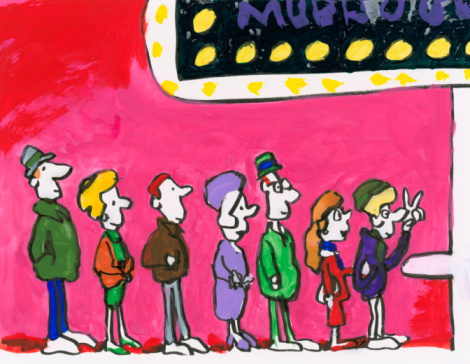
\includegraphics[scale= 0.18]{images/movie.jpg}} \hspace{0.2em}
\onslide<2->{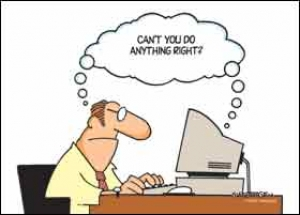
\includegraphics[scale= 0.27]{images/frus.jpg}} \hspace{0.2em}
\onslide<3->{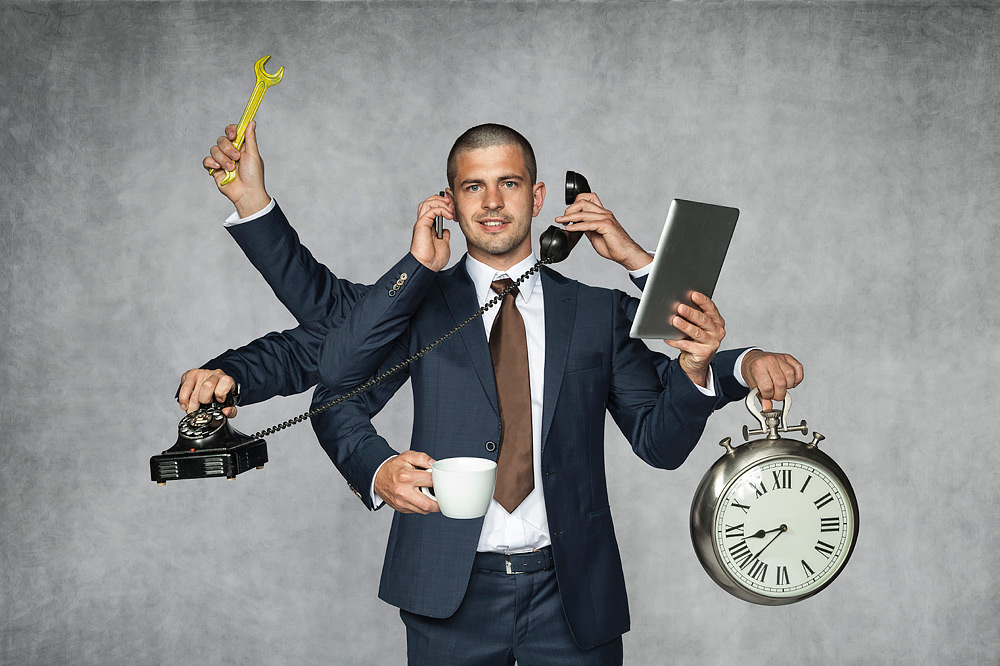
\includegraphics[scale= 0.08]{images/multiple2.jpg}} \hspace{0.2em}
\onslide<4->{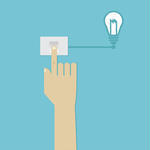
\includegraphics[scale= 1.8]{images/lights.jpg}}\\ \vspace{1.5em}   
\onslide<5->{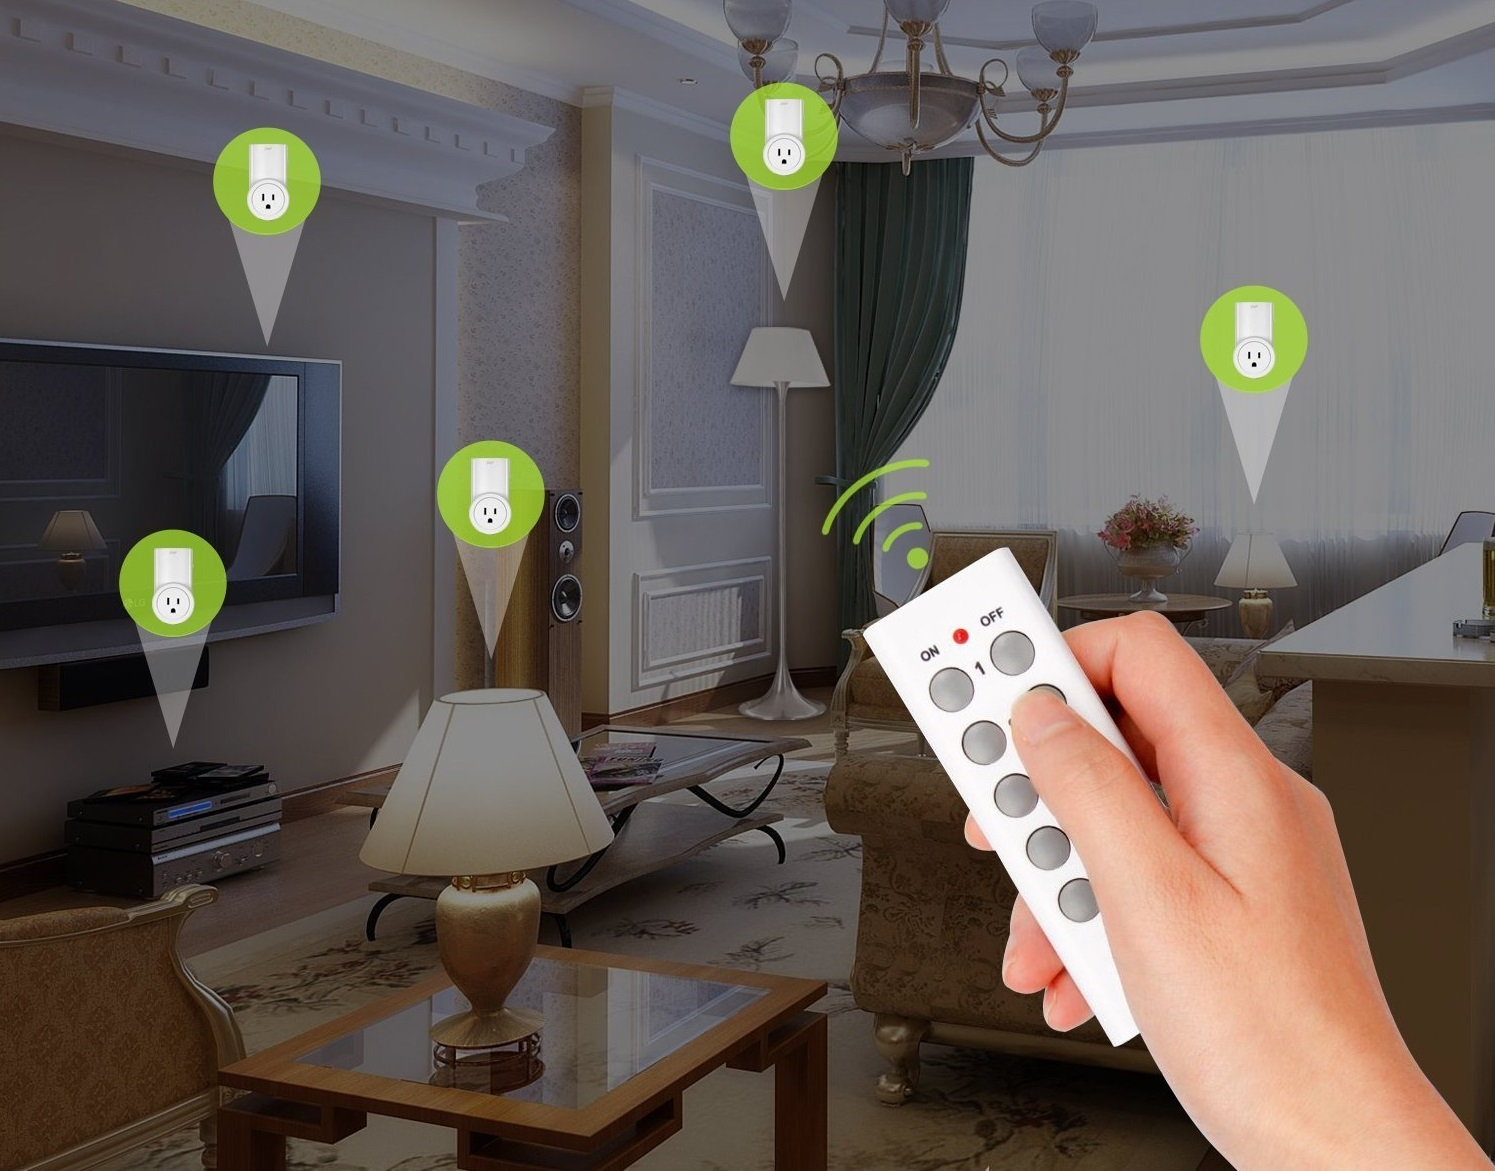
\includegraphics[scale= 0.08]{images/button.jpg}} \hspace{0.2em}
\onslide<6->{
\includegraphics[scale= 0.1]{images/search.jpg}} \hspace{0.2em}
\onslide<7->{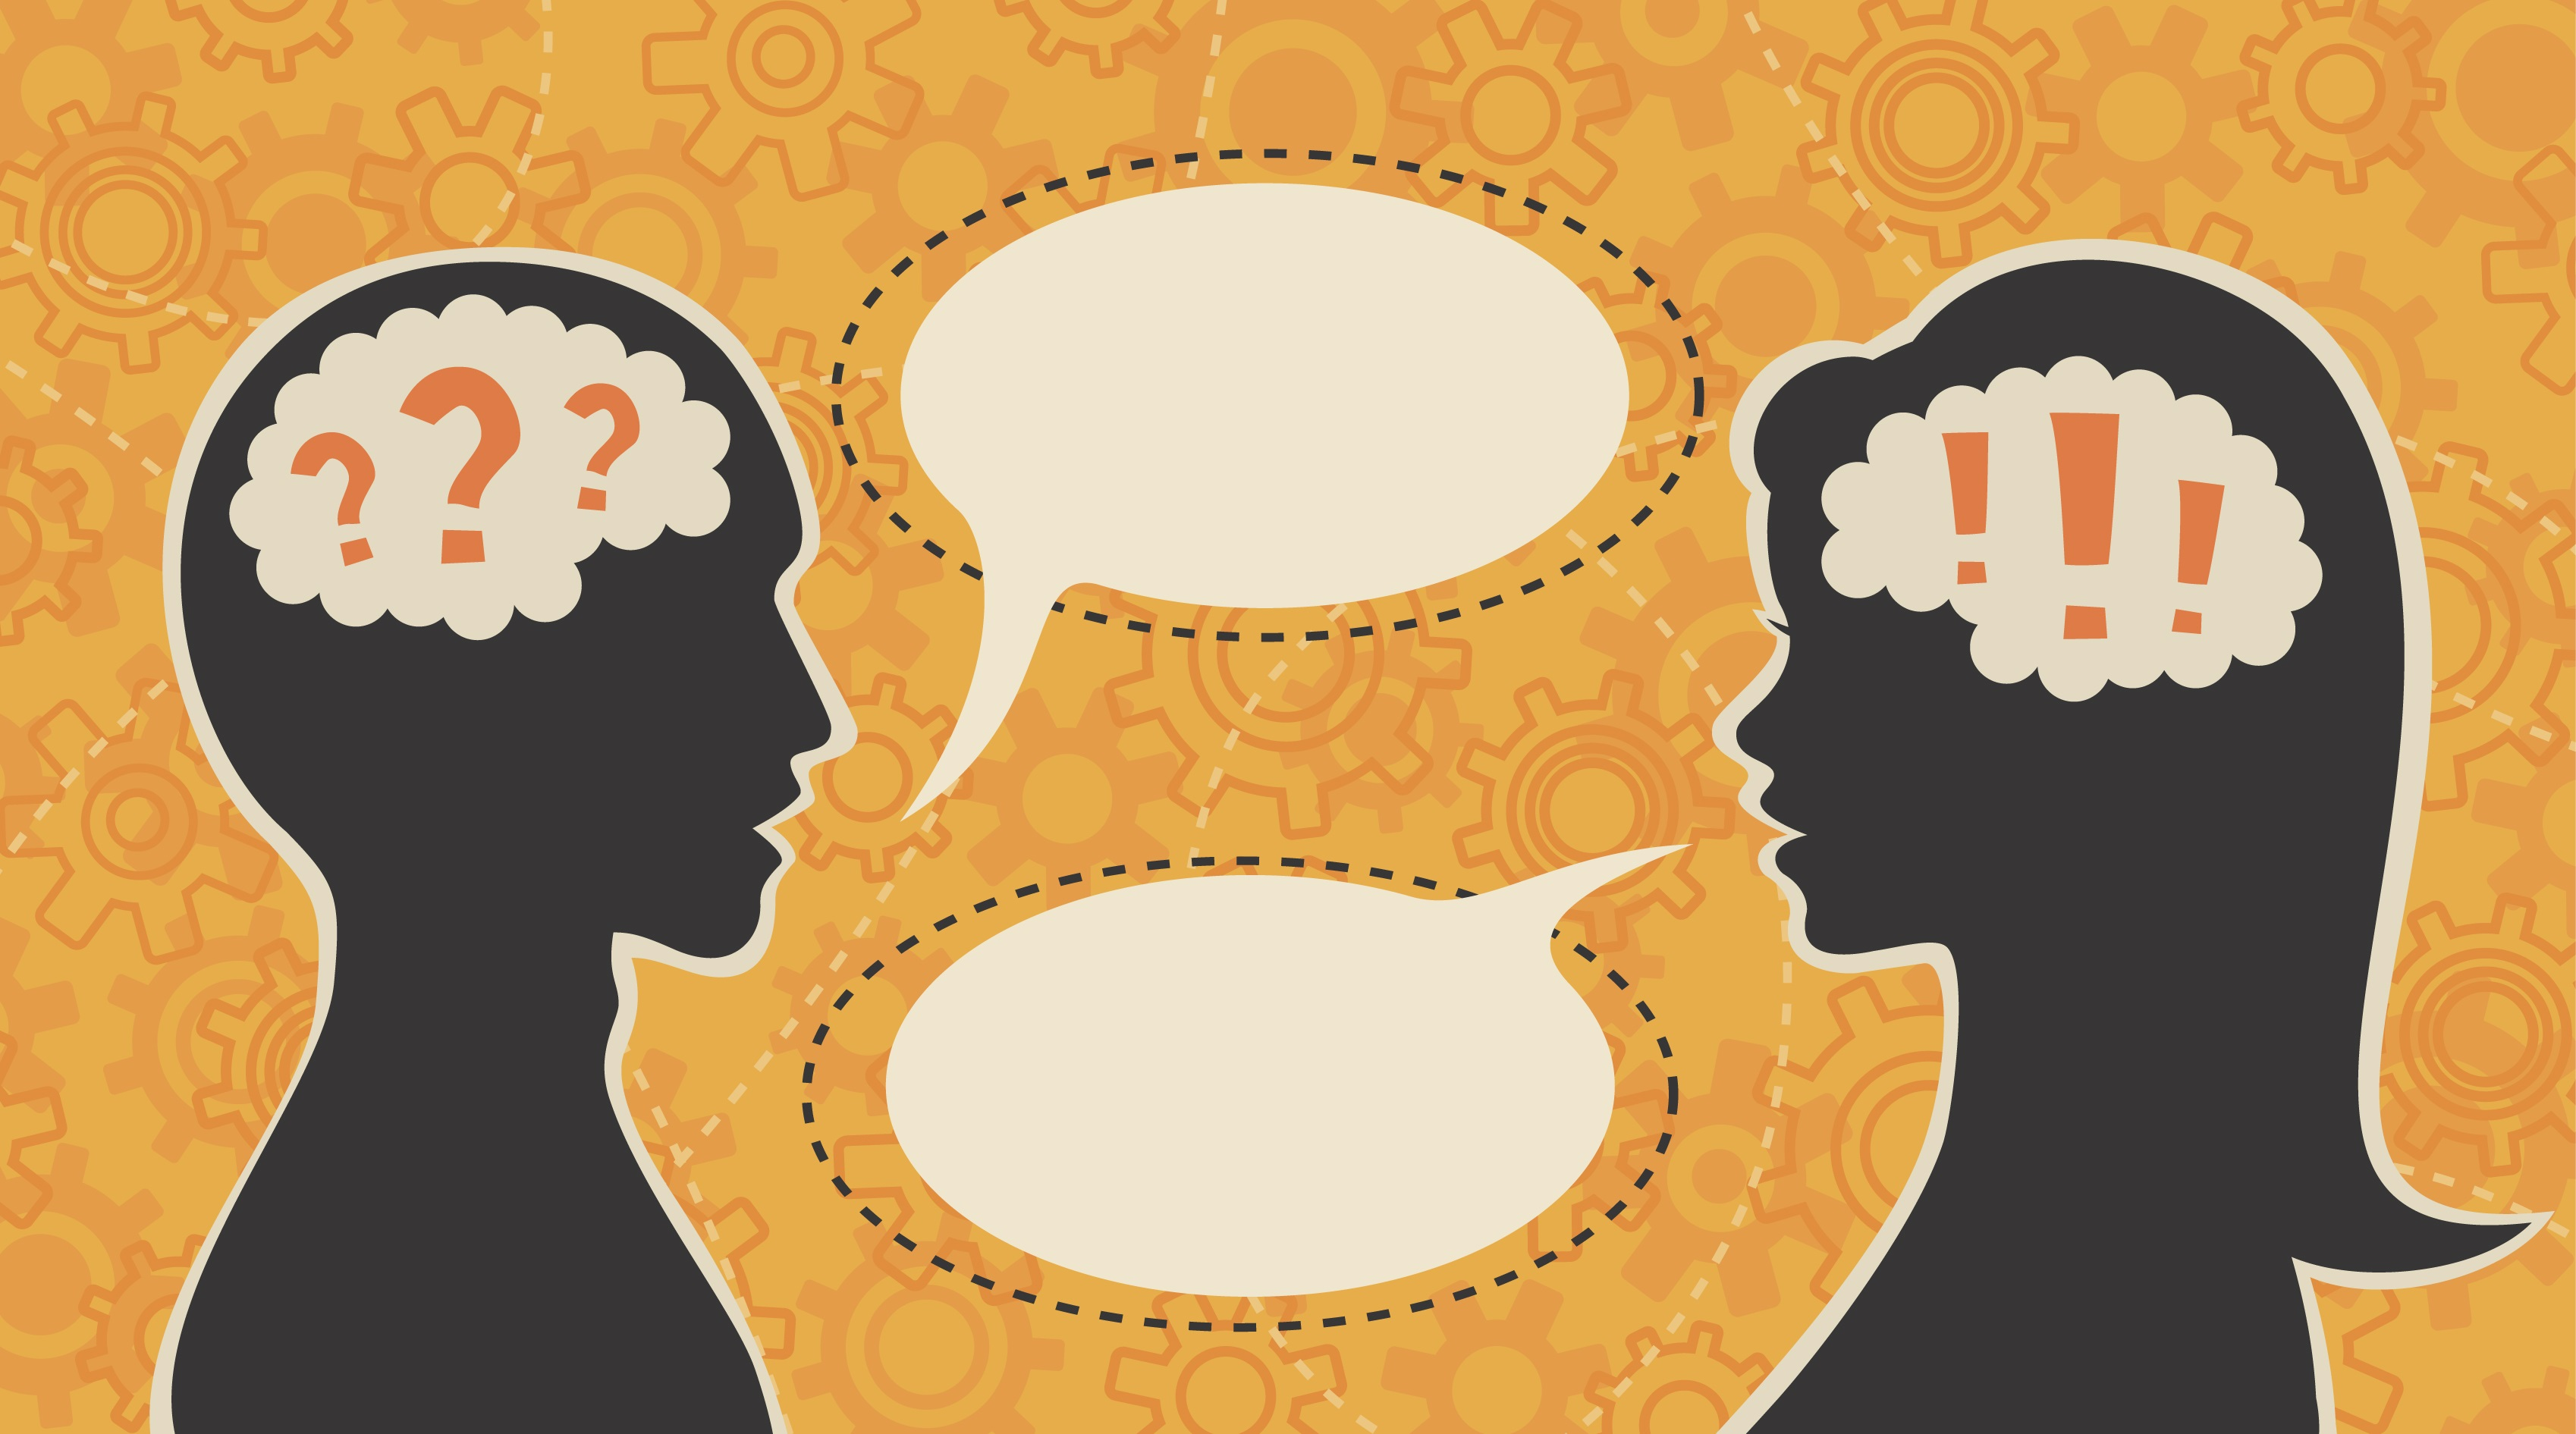
\includegraphics[scale= 0.1]{images/language.jpg}} \hspace{0.2em}
\onslide<8->{
\includegraphics[scale= 0.15]{images/social.jpg}}

\end{figure}
\end{frame}


%------------------------------------------------
\section{Motivation} 
%------------------------------------------------
\begin{frame}
\centering

\includegraphics[scale=0.3]{images/idea.jpg}\\
\vspace{2em}
\textcolor{Blue}{\Huge{\textsf{\textsl{What if we could have one solution to all these problems?}}}}
\end{frame}

\begin{frame}
\frametitle{Motivation}
\begin{figure}
\centering
\resizebox{.6\linewidth}{!}{%
\smartdiagramset{
bubble node size =6cm, 
bubble center node font = \small,
bubble node font = \tiny, 
distance center/other bubbles = 2cm, 
}
\smartdiagramanimated[constellation diagram]{AI Device,Social Network,Intelligent,Answer Basic\\ Questions,Personalized,Connect IOT\\ Devices, Book Tickets,  Identify Images}
}%end resizebox
\end{figure}    
\end{frame}

%------------------------------------------------
\section{Problem Statement}
%------------------------------------------------
\begin{frame} % Need to use the fragile option when verbatim is used in the slide
\frametitle{Problem Statement}
\begin{block}{Statement}
\begin{itemize}
\item To build a Personalised Intelligent Assistant Device that can help humans with the basic task of day to day regimen using their voice.
\item Also to ease the interface of the IOT devices in the surrounding of the Intelligent Device.
\end{itemize}
\end{block}
\end{frame}

%------------------------------------------------
\section{Literature Survey}
%------------------------------------------------
\begin{frame}
\frametitle{Google \small{v/s} \Large{Apache Solr} \small{v/s} \Large{ElasticSearch}}
\begin{table}
\begin{tabular}{l l l}
\toprule
\textbf{Google} & \textbf{Apache Solr} & \textbf{Xapian}\\
\midrule
\tiny{Web Search Engine} & \tiny{Full Text Search Engine} & \tiny{Full Text Search Engine} \\
\tiny{Uses Page Rank for prioritizing} & \tiny{Supports HTTP,XML,JSON} & \tiny{Binding with python,Ruby,Java} \\
\tiny{Stores Location information}& \tiny{Spatial Search Available}&\tiny{No Spatial related Search}\\
\tiny{Not Open Source}&\tiny{Open Source}&\tiny{Open Source}\\
\tiny{Seperates Bold and Larger text from normal}& \tiny{Multi-lingual and synonym Search}&\tiny{Accurate probabilistic Ranking}\\
\tiny{Overuses algorithm, hence fails in medical searches}&\tiny{Slow Startups and Commits}&\tiny{Slow Search due to log search}\\
\tiny{Most used Search engine in WWW}&\tiny{Used by Twitter, LinkedIn, etc.}&\tiny{Debian, Gmane, Die Ziet}\\
\bottomrule
\end{tabular}
\end{table}
\end{frame}

%------------------------------------------------
\section{Introduction}
%------------------------------------------------
\begin{frame}
\begin{center}
\onslide<1->{\textbf{\LARGE{So finally we came up with..!!!}}}\\
\vspace{0.5cm}
\onslide<2->{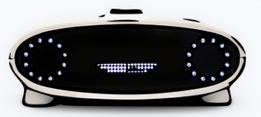
\includegraphics[scale=0.7]{images/mycroft.jpg}}\\
\vspace{0.5cm}
\onslide<3->{\textbf{\LARGE{And we call it}}}
\onslide<4->{\textcolor{Red}{\textbf{\Huge{\hspace{0.5em}{"JASPER"}}}}}
\end{center}
\end{frame}

%------------------------------------------------

\subsection{What is Jasper?}
\begin{frame}[fragile] % Need to use the fragile option when verbatim is used in the slide
\frametitle{What is Jasper?}
\begin{exampleblock}{Introduction}
\begin{itemize}
\item An open source Voice controlled personal assistant device.
\item Written in Python.
\item Built on top of Pocketsphinx STT and espeak TTS.
\item A standalone intelligent device which can perform basic tasks like Web search, Book Tickets, Integrate mails and many more.
\item Can connect the IOT devices in the vicinity and control them with built-in  voice commands.
\item Connects with a Android app to personalize and control the functionality of the device.
\end{itemize}
\end{exampleblock}
\end{frame}
%------------------------------------------------

\subsection{Why use Jasper?}
\begin{frame}[fragile] % Need to use the fragile option when verbatim is used in the slide
\frametitle{Why use Jasper?}
\begin{exampleblock}{Features}
\begin{itemize}
\item Replace the need of having different devices and application for different task performing.
\item Open to community.
\item Skill sets can be extended.
\item Ease of use through voice commands.
\item Can be personalized.
\item Integrated Android Application.
\item Can interface with IOT devices in the vicinity seamlessly. 
\end{itemize}
\end{exampleblock}
\end{frame}
%------------------------------------------------
%------------------------------------------------
%------------------------------------------------

%----------------------------------------------------------------------------------------
\section{Flow Diagram}
\subsection*{Flow Diagram}
%----------------------------------------------------------------------------------------
\begin{frame}
\frametitle{Flow Diagram}
\begin{center}
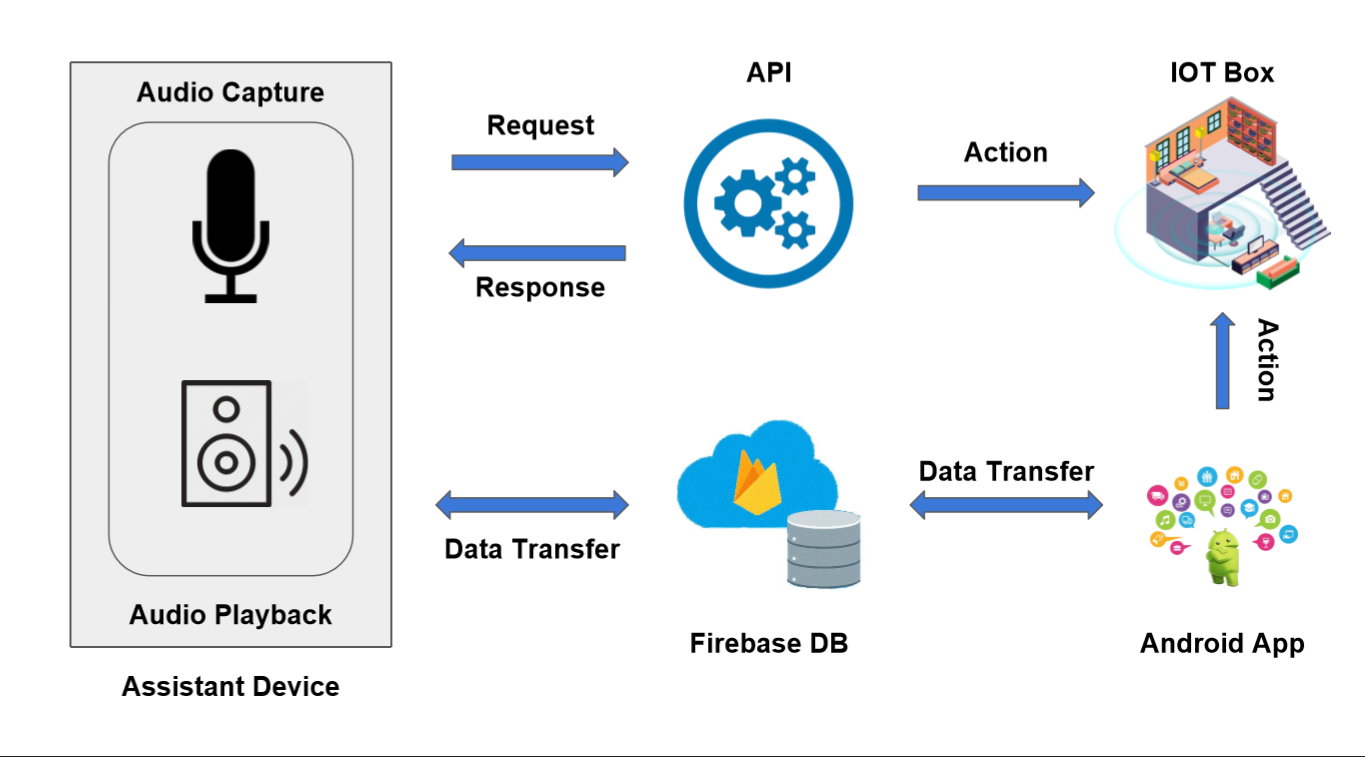
\includegraphics[scale=0.34]{images/Arckin.png}
\end{center}
\end{frame}
%----------------------------------------------------------------------------------------
\subsection*{Detailed Flow Diagram}
%----------------------------------------------------------------------------------------
\begin{frame}
\frametitle{AI Device Flow Diagram}
\begin{minipage}{0.8\textwidth}
\centering 
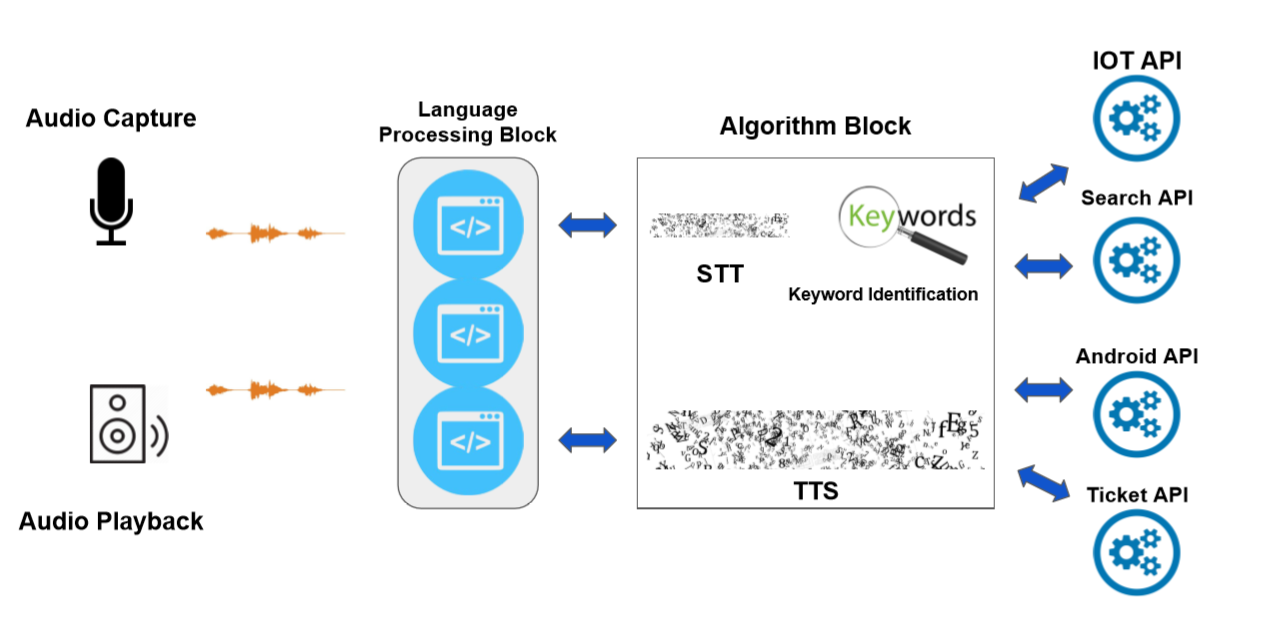
\includegraphics[scale=0.36]{images/Device.png}
\end{minipage}
\end{frame}
%---------------------------------------------------------------------------------------
\begin{frame}
\frametitle{IOT Box Flow Diagram}
\centering
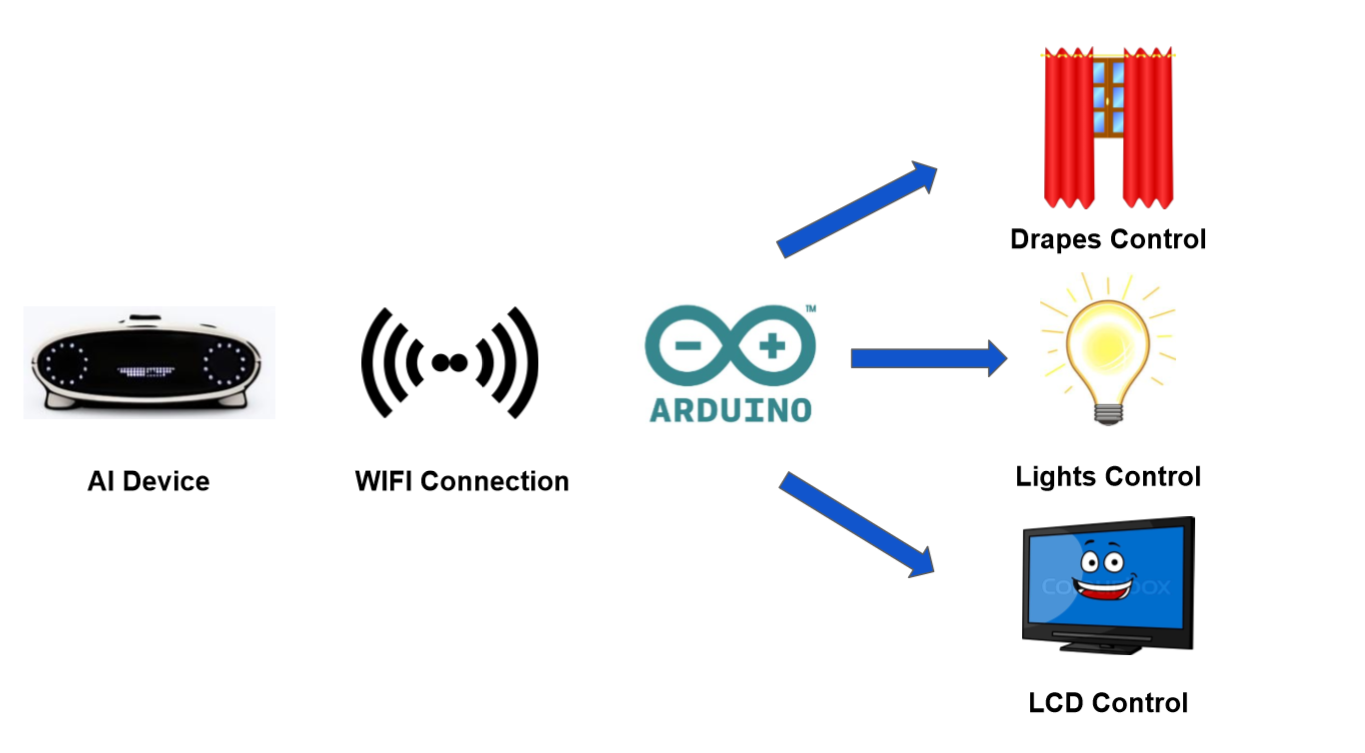
\includegraphics[scale=0.35]{images/IOT.png}
\end{frame}
%----------------------------------------------------------------------------------------
\begin{frame}
\frametitle{Android App Flow Diagram}
\centering
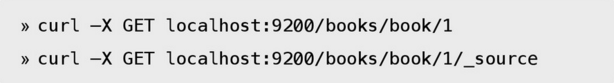
\includegraphics[scale=0.32]{q3.png}
\end{frame}
%----------------------------------------------------------------------------------------
\section{Algorithms}
%----------------------------------------------------------------------------------------
\begin{frame}
\frametitle{Algorithm}
The most prominently used algorithms in ElasticSearch are as follows:
\begin{alertblock}{Algorithms}
\begin{itemize}
\item Relevance Scoring
\item Inverted Index
\item Zen Discovery
\end{itemize}
\end{alertblock}
\end{frame}
%----------------------------------------------------------------------------------------
\subsection{Relevance Scoring}
\begin{frame}[fragile]
\frametitle{Relevance Scoring}
ElasticSearch uses following theories for practical scoring to calculate relevance: 
\begin{columns}[c]
\column{.45\textwidth} % Left column and width
\begin{exampleblock}{\small{Boolean Model}}
The boolean model simply applies the AND,OR and NOT conditions expressed in the query to find all the documents that match.\\
\begin{verbnobox}[\tiny]
full AND text AND(elasticsearch OR Lucene)
\end{verbnobox}
\end{exampleblock}

\column{.45\textwidth} % Right column and width
\begin{exampleblock}{\small{Term Frequency/ Inverse Document Frequency}}
\scriptsize{
\begin{itemize}
\item \textbf{TF}: How often the term appears in the document? More often, Higher the weight.
\item \textbf{IDF}:{\begin{itemize}
\item \scriptsize{How often the term appear in all the documents in the collection? More often, lower the weight.}
\item \scriptsize{How long is field? Shorter the field, Higher the weight.} 
\end{itemize}}
\end{itemize}}

\end{exampleblock}
\end{columns}
\end{frame}
%----------------------------------------------------------------------------------------
\subsection{Inverted Index}
\begin{frame}[fragile]
\frametitle{Inverted Index}
ElasticSearch uses Inverted Index for fast full text-searchs.Let us consider two documents containing respective unique fields:
\begin{enumerate}
\item The quick brown fox jumped over the lazy dog.
\item Quick brown foxes leap over lazy dogs in summer. 
\end{enumerate}
\begin{columns}[c]
\column{.45\textwidth} % Left column and width
\begin{exampleblock}{\small{Inverted Index}}
\begin{center}
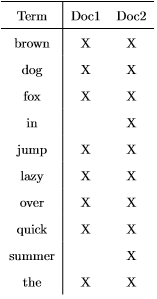
\includegraphics[scale=0.5]{t1.png}
\end{center}
\end{exampleblock}

\column{.45\textwidth} % Right column and width
\begin{exampleblock}{\small{Weight Calculation for the summer}}
\begin{center}
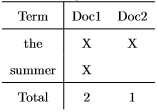
\includegraphics[scale=0.5]{t2.png}
\end{center}
\end{exampleblock}
\end{columns}
\end{frame}
%----------------------------------------------------------------------------------------
\subsection{Zen Discovery}
\begin{frame}
\frametitle{Zen Discovery}
\begin{center}
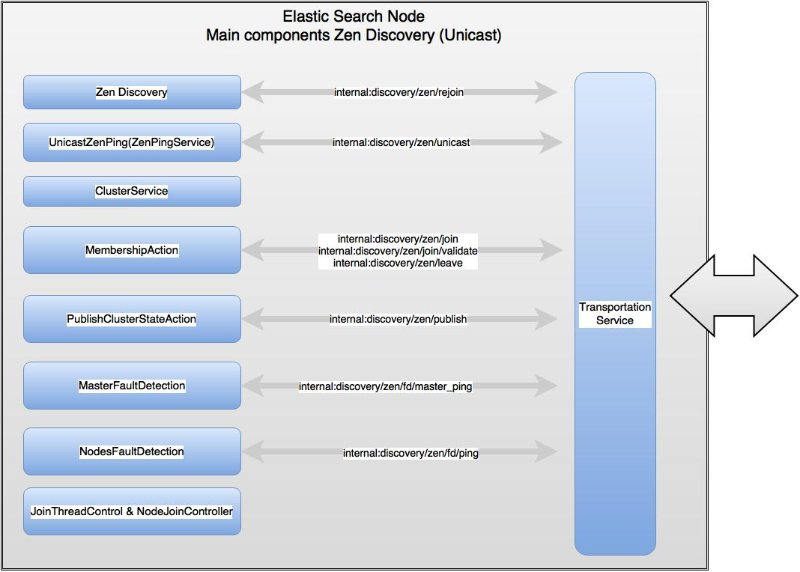
\includegraphics[scale=0.34]{zen.jpg}
\end{center}
\end{frame}
%----------------------------------------------------------------------------------------
\section{Advantages}
%----------------------------------------------------------------------------------------
\begin{frame}
\frametitle{Advantages}
\begin{exampleblock}{Advantages}
\begin{itemize}
\item \textbf{Built on top of Lucene}: It stores real world complex entities as JSON Documents and indexes them by default.
\item \textbf{Full-text Search}: It supports full text search along with spatial search and tokkening and customizing the search.
\item \textbf{Schema Free}: It accepts the JSON Documents and tries to detect the data structure and further adds the fields if not present. The fields can also be dropped.
\item \textbf{RESTful API}: Searhc is API Driven.
\item \textbf{Open Source}: All the documentation related to Elastic Search are Open for public.
\end{itemize}
\end{exampleblock}
\end{frame}
%----------------------------------------------------------------------------------------
\section{Conclusion}
%----------------------------------------------------------------------------------------
\begin{frame}
\frametitle{Conclusion}
\openup 0.7em
Elastic Search allows to store, search and analyze huge amount of data quickly and in near real time.\\ It is a great open source tool built on top of LUCENE but uses JSON+RESTful API.\\ Also it is easy to setup and get started with.\\ And it is dynamically load balances just like Google does. 
\end{frame}
%----------------------------------------------------------------------------------------
\section{Future Scope}
%----------------------------------------------------------------------------------------
\begin{frame}
\frametitle{Future Scope}
\begin{alertblock}{Future Scope}
\begin{itemize}
\item To create zones within the cluster and and newly created shards are allotted to highly- ended zones and older shards are shifted to lower-ended zones. Hence lower ended zone have to provide much greater relevance during ranking which improves the search output.
\item Shard selection is highly advantages till it is used in web searching. As it comes down to enterprises search where shards can be structured, shard selection proves costly at times.
\item Automatically scaling can also be integrated in future. 
\end{itemize}
\end{alertblock}
\end{frame}
%----------------------------------------------------------------------------------------
\section{References}
%----------------------------------------------------------------------------------------
\begin{frame}
\frametitle{References}
\begin{thebibliography}{5}
\bibitem{beamer} \emph{ Nil Goksel-Canbek ,Mehmet Emin Mutlu: On the track of Artificial Intelligence: Learning with Intelligent Personal Assistants , 2016.}{\vspace{.6cm}}
\bibitem{beamer2} \emph{Harshita Phatnani, Mr. Jyotiprakash Patra, Ankit Sharma: An Intelligent Voice Assistant Using Android Platform , 2016 }{\vspace{.6cm}}
\bibitem{beamer2} \emph{Vinay Sagar, Kusuma SM:Home Automation Using IOT , 2015 }{\vspace{.6cm}}
\bibitem{beamer2} \emph{ Douglas OShaughnessy, Senior Member: Interacting With Computers by Voice: Automatic Speech Recognition and Synthesis,2003}{\vspace{1cm}}
\end{thebibliography}
\end{frame}
%----------------------------------------------------------------------------------------
\begin{frame}
\begin{center}
\textbf{\huge{That's It\\\vspace{0.2cm} Thank You}}\\
\vspace{0.5cm}

\includegraphics[scale=1.5]{thank.jpg}
\end{center}
\end{frame}
%----------------------------------------------------------------------------------------
\end{document} 
